 \documentclass{article}
\usepackage[a4paper]{geometry}
\usepackage[version=3]{mhchem} % Package for chemical equation typesetting
\usepackage{graphicx} % Required for the inclusion of images
\graphicspath{ {Images/} }
\geometry{tmargin=2.5cm,bmargin=2.5cm,lmargin=2.5cm,rmargin=2.5cm}
\usepackage{subfig}
\usepackage{float}
\usepackage{natbib} % Required to change bibliography style to APA
\usepackage{amsmath} % Required for some math elements 
%\usepackage[authoryear]{natbib}
\usepackage{algorithm}
\usepackage{algorithmic}

%\setlength\parindent{0pt} % Removes all indentation from paragraphs

%\renewcommand{\labelenumi}{\alph{enumi}.} % Make numbering in the enumerate environment by letter rather than number (e.g. section 6)

%\usepackage{times} % Uncomment to use the Times New Roman font



%----------------------------------------------------------------------------------------
%	DOCUMENT INFORMATION
%----------------------------------------------------------------------------------------

\title{Scene Segmentation and Interpretation\\Coursework 2. Image Characterisation using Texture} % Title

\author{Fl\'{a}via \textsc{Dias Casagrande} and Dragutin \textsc{Vujovic}} % Author name

\date{\today} % Date for the report

\begin{document}

\maketitle % Insert the title, author and date


%----------------------------------------------------------------------------------------
%	SECTION 1
%----------------------------------------------------------------------------------------

\section{Objective}

This report presents all the implementation of one of the most common statistical methods in order to extract texture descriptors, the co-occurrence matrices, developed in Matlab.

%----------------------------------------------------------------------------------------
%	SECTION 2
%----------------------------------------------------------------------------------------

\section{Introduction and problem definition}

Image characterization consists in obtaining properties that
represent regions of the image. It can take in account several criteria, such as color, shape and texture.

The executed lab is based on the later. Texture can be seen as a repetitive pattern on a surface. Analysing the different textures in an image could be done for many purposes, such as texture classification and image segmentation, both implemented in this lab.

There are many methods in order to perform texture extraction: statistical, structural, modelization and space frequency filtering. The statistical methods was the implemented one, which takes in account the spatial distribution of gray values by computing local features at each point in
the image, and then calculating statistics from certain distribution. Specifically, the method used was the co-occurrence matrices.

The co-occurrence method consists in computing the probability of finding two pixels with certain values in a direction in a window. Then some statistic descriptors such as energy, contrast, homogeneity, correlation, etc., are computed.

The goal of the lab is then to calculate these texture descriptors by using the Grey Level Co-occurrence Matrix (GLCM). This is done in a local scale, which means each pixel will have own statistical descriptors provided by GLCM.

A second part in the lab is to calculate the descriptors globally. A vector with the descriptors calculates for each image is defined and a texture classification step is performed.

\section{Texture algorithm analysis}


The GLCM is a matrix that represents how often different combinations of pixel intensity values (grey levels) occur in an image.

Each pixel in the image will have a matrix, and for this calculation, a window  should be defined around it. The window should be big enough to capture the texture properties.

After the matrix is normalized, it represents the probability that two points with grey-levels i and j exist in a distance d and orientation $\theta$. Figure \ref{fig:coc} illustrates how the co-occurrence matrix would be defined for the corresponding subimage. Taking a distance of 1 pixel, and orientation of 90 degrees (since it is a bidirectional orientation, angles of 180 degrees are also taken in account).

\begin{figure}[h!]
  \centering
    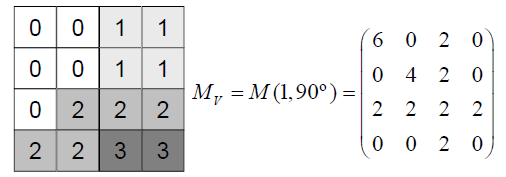
\includegraphics[width=0.5\textwidth]{coc}
    \caption{Example of co-occurrence matrix, extracted from class lectures.}
    \label{fig:coc}
\end{figure}

Once the co-occurrence matrix is computed for each pixel, the statistics can be derived. For this lab, the following were used: energy, homogeneity, contrast and correlation.


\section{Design and implementation of the proposed solution for the segmentation problem}

The texture characterization algorithm described in the previous section was implemented and its pseudo-code can be seen below.

\begin{algorithm}
\caption{Texture Segmentation}
\begin{algorithmic} 
\STATE $\textit{Chose size of window}$
\STATE $\textit{Execute image padding}$
\STATE $\textit{Initialize result matrix - same size as image 3}$
\FOR{ $\textit{each pixel (i,j) in image}$}
\STATE $\textit{Compute co-occurrence matrix M in position (i,j)}$
\STATE $\textit{Compute statistics from M}$
\ENDFOR
\STATE $\textit{Perform region growing algorithm in result matrix}$
\end{algorithmic}
\end{algorithm}

More in details, the code written has only one function called \textit{textureSegmentation}. It receives the image path and the window size for the calculation of co-occurrence matrix.

The image is then loaded (\textit{imread}), passed to gray level (\textit{rgb2gray}) and padded with zeros. Four matrices are initialized, corresponding to each calculated descriptor: energy, contrast, entropy and homogeneity.

Then, there are two \textit{for loops} in order to pass through all the pixels in the image. For each pixel, its co-occurrence matrix is calculated by using the function \textit{graycomatrix}. The result is passed to the function \textit{graycoprops}, which returns the desired descriptor. This function has already the option to choose between the mentioned descriptors, or simply all of them. Each one can be accessed then and assigned to the corresponding matrix.

For the segmentation, the function developed in the first coursework was used, called \textit{growingRegion}. It gets as parameters the image, the connectivity to be taken in account and the desired threshold.


\section{Experimental section and results analysis for the segmentation problem.}


Is the use of texture useful? What are the limitations?

%\begin{figure}[h!]
%  \centering
%    \includegraphics[width=1\textwidth]{gantry}
%    \caption{Gantry image segmentation - threshold of 30.}
%    \label{fig:gantry}
%\end{figure}




\section{Design and implementation of the proposed solution for the classification problem}

For the classification, two functions were already provided \textit{scr\_classify} and \textit{scr\_classifyPR}. The only implemented function was the \textit{computeFeatureVector}. It follows the pseudo-code.

\begin{algorithm}
\caption{Texture Classification}
\begin{algorithmic} 
\STATE $\textit{Initialize result matrix - same size as image 3}$
\STATE $\textit{Compute co-occurrence matrix M for image}$
\STATE $\textit{Compute statistics from M}$
\STATE $\textit{Define a vector with statisticis calculated}$
\end{algorithmic}
\end{algorithm}

More specifically in the case of the code written, the function \textit{graycomatrix} is used in the whole image at a time (global), and right after the \textit{graycoprops} function, to calculate the descriptors.

Each value is put in a vector that will be used by the given functions. The provided functions extract the features of the training and testing sets, by using ``Random Forests" classifier from the weka library. The output is the confusion matrix and the percentage of the correct classification.

For a perfect classifier, the confusion matrix should have numbers only in the diagonal.

\section{Experimental section and results analysis for the classification problem.}


\section{Organization and development of the coursework}

The tasks for executing the coursework were quite simple and sequential. First the development of the GLCM locally and posterior segmentation (which was only use the function implemented in Coursework 1). This first part took two hours. After that, the texture classification step was implemented, which took also two hours. When all the algorithms were working correctly, the interface was developed (two hours). The last task was the report writing (four hours).

The real dedication for this coursework was then of ten hours. The estimated time dedication for this coursework is four hours (two lab sessions).  As the interface was not a requirement, we could say the time estimated for the lab execution was the real one, plus the time for the report.


\section{Conclusions}

The GLCM produced good results for some images and not so good for others. It depends of many parameters

We understand texture extraction as a good image segmentation analyser, but it would be much better if used with other features such as color and shape, for example.

Regarding the time necessary for the algorithm to run, GLCM is very time consuming. Naturally, it is even slower when applied for every pixel in the image, requiring then two \textit{for loops}.

It was a really nice lab to understand the texture extraction and classification algorithms, combining it with the previous lab of segmentation.

\end{document}

